
\chapter{Static gestures recognition}

As was already mentioned, the detected gestures can be divided into two groups: static gestures and dynamic gestures.
The static gestures can be understood as a chosen position and orientation of the fingers and hand in a single moment, while dynamic gestures are defined as a movement of the hand and fingers in time. 
The problem of recognition of those gestures is a subject of following chapter. 
Firstly, the proposed approach is presented, followed by the introduction to the evaluation scheme. 
In last section, the performed experiments are descriebed, which were used to examine the effectiveness of proposed static gesture recognition approach.

\section{Proposed methods}

The static gesture recognition problem can be stated as a problem invariant to time.
That means that for each detected hand, the position and orientation can be treated as a new data uncorrelated to previously classified data.
While this assumption means that one can easily generate multiple samples from the sensors in short time, it also gives an opportunity to look at the static gesture recognition problem as a problem of classification.

While for most 2D gesture recognition problems simple classification algorithms seems to work well enough, the 3D data is more complication to model by the set of features and finally successfully label.
While dealing with 3D data, the position and orientation of hand can be easily affected by the height of the hand above the sensor or small change in the orientation of the hand with respect to the sensor's coordinate system. 
It is intuitively understood, that the system should recognize those gestures as the one as they are similar.
To meet those requirement, one need to define what is meant by the ,,small'' change in orientation resulting in treating the static gestures as the same.

\begin{figure}[htb]
\centering
 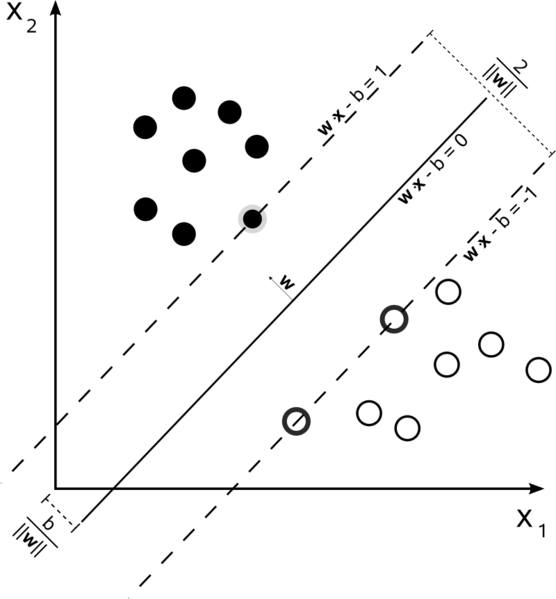
\includegraphics[width=0.6\columnwidth]{figures/SVM.png}
 \caption[]{SVM is a technique searching for the hiperplane that maximizes the margin between classes\footnotemark}
 \label{svmmargin}
\end{figure}



To meet those requirements, the Support Vector Machines \cite{Cortes:SVM} were used as a classification algorithm.
The SVMs were chosen as there exist a solid mathematical background supporting the simple idea of maximalizing the margin between classes.
Moreover, the SVMs were chosen also because of the popularity due to the open-source library libSVM \cite{libSVM}, which contains the multiple platform SVM implementation.
It is worth noticing that in original work, SVMs were used only to classify between two classes, but the idea was expanded to utilize the one-vs-all scheme allowing to classify multiple class sets.
The efficiency of SVMs depends on correctly choosing the kernel function used to map the separation problem into higher-dimension with expectation to achieve problem easier to solve.
The typical kernel functions:
\begin{itemize}
\item linear: $K(x_i, x_j) = x_i^Tx_j$.
\item polynomial: $K(x_i, x_j) = (\gamma x_i^Tx_j + r)^d, \gamma > 0$.
\item radial basis function (RBF): $K(x_i, x_j) = exp(-\gamma ||x_i - x_j||^2), \gamma > 0$.
\item sigmoid: $K(x_i, x_j) = tanh(\gamma x_i^Tx_j+r)$.
\end{itemize}
where $\gamma$, $r$, and $d$ are kernel parameters. According to the authors of the library, linear kernels should be used for linearly separable problems, while RBF kernel is the most versatile one.

\footnotetext{\url{http://en.wikipedia.org/wiki/File:Svm_max_sep_hyperplane_with_margin.png}}

The problem of classification assumes that each sample consists of set of features, which describe this sample and can be used to distinguish it from the other samples.
Additionally, each sample has a known or unknown label, which defined the membership of sample to the class. 
The samples with the known labels can be used to train the classification system to compute the membership to the classes for the samples. 
The computation is performed on previously mentioned sets of features.

In application of gesture recognition the classification be divided into two flows: the training part and the recognition part. 
In training part, the library will be provided with the samples of static gestures with known correspondences to the static gesture classes. 
From those samples, the sets of features are computed, which are used to train the classifier.
The recognition part assumes to have trained classifier. 
The recognition part is provided with samples static gestures without labels. 
For each sample the sets of features are computed and then given as input to the trained classifier.
The classifier returns the information of the gesture's class membership (label) of each sample.

In case of library, it is assumed that the learning process can be done offline, while strict online requirements has to be met in recognition part. 
To meet those requirements the Support Vector Machine is introduced\cite{Cortes:SVM}. 
The SVM classification is commonly used technique in multiple areas of research as biology, robotics or IT for solving data classification problems.
Additional advantage of the SVM is possibility to use C++ library libSVM \cite{libSVM}, which provides an easy interface to utilize this classification methods in different problems.

\begin{figure}[htb]
\centering
 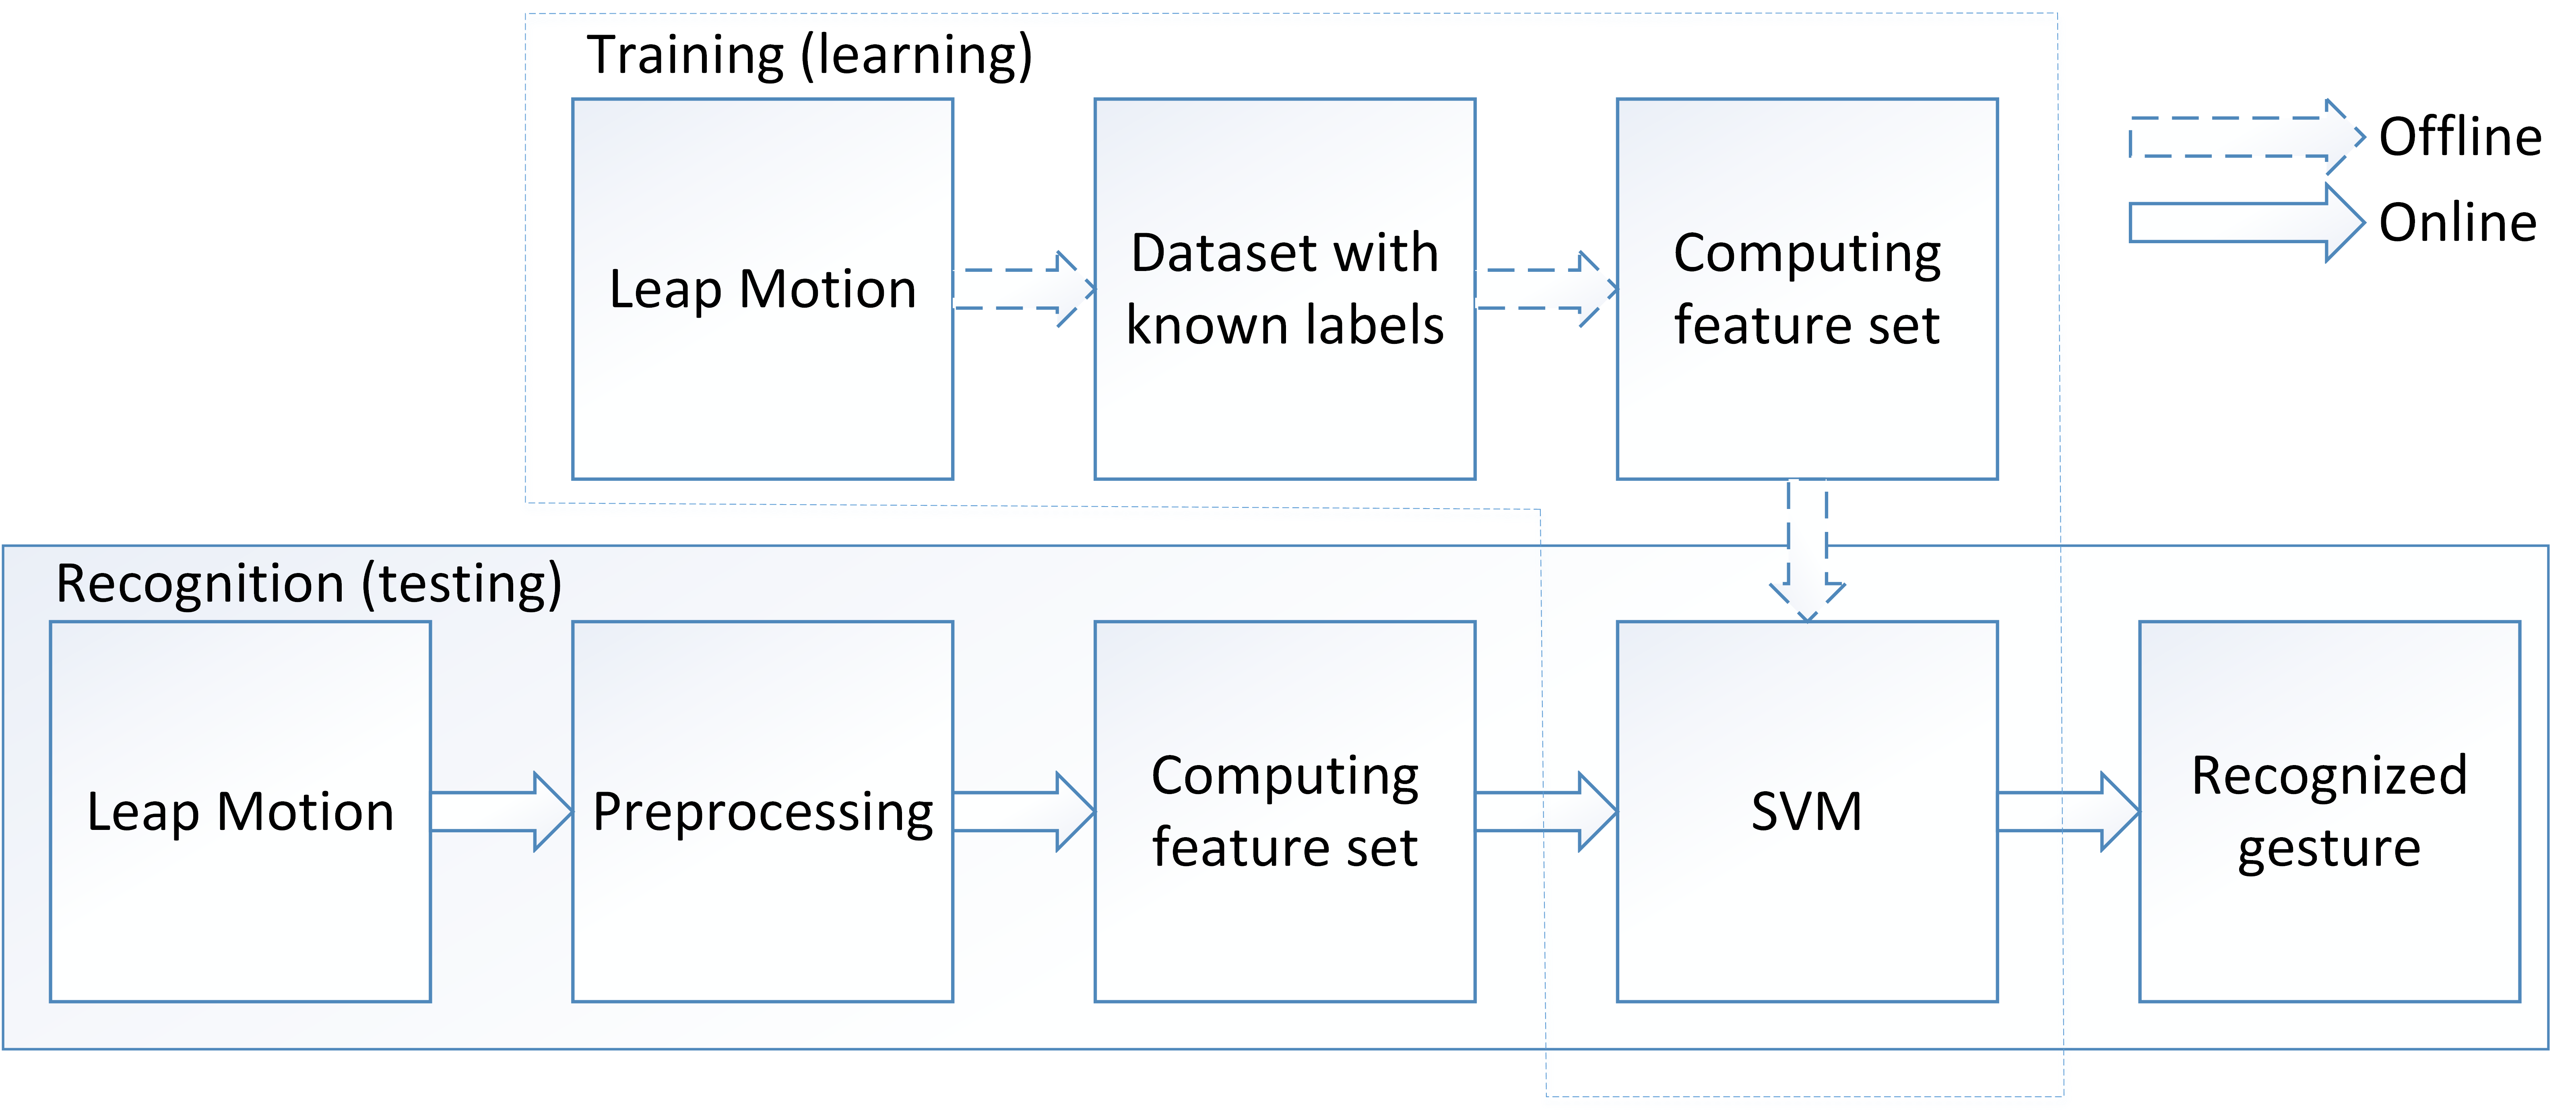
\includegraphics[width=1\columnwidth]{figures/StaticGestures.png}
 \caption[]{Proposed solution blocks for learning and recognition parts of static gestures recognition problem}
 \label{staticsol}
\end{figure}


While presented approach can be treated as state-of-the-art approach it still cannot be used without defining proper feature sets for gesture recognition.
The naive solution would be to use the raw data from Leap motion sensor as the feature set.
This solution was tested, but provided poor results as the proposed features were dependent on the position, orientation and scale of hand. 
Even small movement in any direction meant problems with stable recognition. 
The theoretical literature suggests to compute a set of features invariant to wanted transformations, which can allow to fully distinguish between different classes.
Unfortunately, there are not available propositions to feature sets when it comes to the gesture recognition using the data even similar to the data provided by the Leap Motion sensor.
Seeking right feature is a task undertaken in experimental section~\ref{static:exp}.

To sum up, the static gesture processing flow is presented at fig.~\ref{staticsol}. In training part, the data from Leap Motion is preprocessed, the feature sets are computed and the data is used to train SVM classifier.
In recognition part, the data is also preprocessed and described by the feature sets, but the knowledge of the label comes from the already trained SVM classifier.


\section{Evaluation methodology}

\subsection{Assumptions}
To provide user with library working in different conditions, it was assumed that the gesture is treated as the same one independently with respect to the translation, rotation and scale of the hand. 
This assumption means that the static gesture rotated by unknown angles, translated in sensor coordinate system and also with different hand sizes should still be recognized as the same gesture.
Invariance to the rotation, translation and scale poses a great challenge to the recognition, but allows the future users of API to fully utilize the feasibility of the library.
It is worth mentioning that, it does not reduce the possible applications of the library, as an assignment of static gesture to already defined class allows to find the transformation between the model of the class and observed gesture.


\subsection{Recorded datasets}

To propose and test the quality of the features twelve static gestures were chosen:
\begin{enumerate}
\item the peace sign,
\item a fist,
\item full hand with space between each finger,
\item American Sign Language: ``I love you'' sign,
\item sign ``gun'' created by putting thumb and forefinger up, while holding the rest fingers in a fist,
\item all fingers in a fist with exception of thumb, which is up,
\item the sign X made with the forefingers of both hands,
\item the sing ``Time'' used e.g. by coaches in basketball games.
\item sign simulating rotating a knob by two fingers,
\item sign simulating rotating a knob by five fingers.
\end{enumerate} 

\begin{figure}[htb]
\centering
 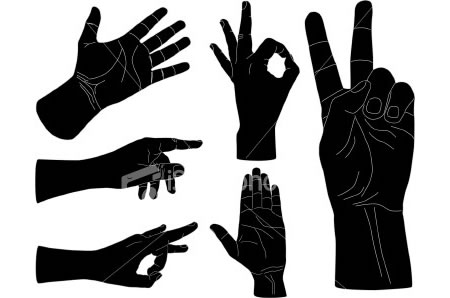
\includegraphics[width=1.0\columnwidth]{figures/static_gestures.png}
 \caption{Recorded static gestures used for evaulation}
 \label{staticgesturesdata}
\end{figure}


The gestures are also presented at fig.~\ref{staticgesturesdata}.


The sample data of each gestures were recorded using the continuous mode of recording, while moving the hands in different directions and changing the orientation of the hands. 
For each of the proposed gestures, each author recorded approximately 1000 samples.

Having samples with known labels, the whole dataset was separated into training and testing sets in relation $2:1$. 
For the training, the k-fold cross-validation (CV) scheme was used, which searches for optimal $C$ and $\gamma$ parameters trying to prevent the algorithm from over-fitting the training data.
This method is used to find the optimal parameters of the classification system, while estimating the performance on the data not used in the training part. 
In standard version of the method, the gathered data is divided into two sets: one containing k-1 parts of the data, the other 1 part of the data. 
The first is used to train the classification system, while the rest of the gathered data is used to estimate the performance. 
The performance is estimated by calculating the number of cases when the classification system returned a label which matched already known label. 
The percent of correctly recognized labels to the total size of the testing set is known as recognition rate.


\section{Experiments}
\label{static:exp}

Firstly, the experiments to find the proper set of features were conducted. The first proposed vector of features consisted of:
\begin{itemize}
\item number of fingers in frame,
\item the euclidean distance between consecutive finger's tips,
\item the absolute angles between consecutive fingers.
\end{itemize} 

While this feature set did not take into account the relative position of fingers to the hand, the second and third feature set were introduced.
The second feature set is a first feature set extended by the distances between consecutive finger tips and the position of the hand's palm.
The third feature set contains features from second feature set extended by the five angles between fingers and normal of hand's palm.
Those, 3 proposed feature sets were firstly tested on all $10$ recorded static gestures.
The firstly tested set of all static gestures contained gestures, which were undistinguishable for the Leap Motion, because they did not take into account the way how the Leap Motion works. 
For gestures like fist or 'X' the recorded data contained almost no information how to classify those gestures.
That's why the experiments were repeated on the five gestures, which could be easily distinguish using the data provided by Leap Motion. 
For this experiment the gestures peace, hand, ''I love you'', fist with thump up and rotating knob by 5 fingers were chosen.
The results achieved by those methods are presented in the table~\ref{staticfeat}.

\begin{table}[htp!]
	\label{staticfeat}
	\caption{Results obtained by experimental feature sets by the libSVM library}
    \begin{tabular}{|c|c|c|c|c|}
    \hline
    ~                                                   & 5 gestures, CV & 5 gestures, test set & 10 gestures, CV  & 10 gestures, test set \\ \hline
    feature set 1                     & ~      & ~           & ~       & ~           \\ \hline
    feature set 2                     & ~      & ~           & ~       & ~          \\ \hline
    feature set 3                     & ~      & ~           & ~       & ~           \\ \hline
    feature set 4                     & ~      & ~           & ~       & ~           \\ \hline
    feature set 5                     & ~      & ~           & ~       & ~          \\ \hline
    feature set 6                     & ~      & ~           & ~       & ~           \\ \hline
    \end{tabular}
\end{table}

After approach allowed to achieve XXX\% of recognition rate and could be unsatisfying from the perspective of the purpose of the application. 
Analysis of the finger numbering revealed that the fingers are numbered accordingly to the position in Z axis of the tip of the finger.
This means that when features are approximately on the same position in Z axis, the numbering can change rapidly and proposed features are computed between different fingers.
To achieve features that would be invariant to the numbering of the fingers, the feature set was slightly modified.
Instead of containing the absolute angles and distances between consecutive fingers, it was proposed to contain the five greatest values of angles and five greatest values of distances between all combinations of finger pairings.
The same sorting approach was used for the angles and distances between fingers and hand's palm.
The feature sets 1, 2, 3 with sorting scheme were respectively called feature sets 4, 5, 6.
Again, the same dataset with 5 and 10 gestures was used to evaluate those methods. 
The results are yet again presented in table~\ref{staticfeat}.
This approach was tested on the same training set and allowed to increase the recognition rate to the XXX\%.

\begin{table}[htp!]
\begin{center}
	\label{staticfeatlin}
	\caption{Results obtained by experimental feature sets by the libLinear library}
    \begin{tabular}{|c|c|c|c|c|}
    \hline
    ~                                                   & 5 gestures, CV & 5 gestures, test set & 10 gestures, CV  & 10 gestures, test set \\ \hline
    feature set 1                     & 78.282\% & 78.283\%  & 50.596\% & 50.593\% \\ \hline
    feature set 2                     & 78.282\% & 78.283\%  & 50.596\% & 50.593\% \\ \hline
    feature set 3                     & 78.282\% & 78.283\%  & 50.596\% & 50.593\% \\ \hline
    feature set 4                     & 78.205\% & 78.242\%  & 50.658\% & 50.575\% \\ \hline
    feature set 5                     & 79.527\% & 79.502\%  & 55.284\% & 55.263\% \\ \hline
    feature set 6                     & 88.0756\% & 88.138\% & 64.747\% & 64.830\% \\ \hline
    \end{tabular}
    \end{center}
\end{table}

While using more data, it is worth noticing the growth of training time. 
In case of $5000$ training samples the typical training process took approximately 12 hours on standard desktop PC. 
This computing time can be unacceptable by the users of the library, so the test with another SVM library libLinear~\cite{libLinear} was performed. 
The libLinear's implementation of SVM utilizes the linear kernels, which are useful for large data training sets with multiple number of features. 
This library reduced the training time to about 5 seconds, but the best obtained recognition rate was smaller in case of libLinear library when compared to the libSVM.
For the 5 gesture case, the libLinear achieved 88.138\% on testing set while using feature set 6 compared to the XXX\% achieved by libSVM in the same condition.
Similarly, in 10 gesture case, libLinear achieved 64.830\% compared to XXX\% by LibSVM.
All achieved results are presented in tab.~\ref{staticfeatlin}.
From the results obtained by the libSVM and libLinear on different feature sets, the feature set 6 was chosen as the one yielding the best results and used in further analysis.

Another factor, that might have an influence on the results is the preprocessing part. 
The preprocessing operates in the window of hands poses, which size can be modified. 
For these reason, the experiments with no preprocessing and preprocessing with width size equal to 5, 10, 15 were performed and the influence on the recognition rate was examined.
The results are presented in tab.~\ref{staticpre}.


\begin{table}[htp!]
\begin{center}
	\label{staticpre}
	\caption{The recognition rate achieved with feature set 6 and different parameters of preprocessing}
    \begin{tabular}{|c|c|c|c|c|}
    \hline
    preprocessing                                                   & 5 gestures, CV & 5 gestures, test set & 10 gestures, CV  & 10 gestures, test set \\ \hline
    off                     & x\% & x\%  & x\% & x\% \\ \hline
    width = 2                     & x\% & x\%  & x\% & x\% \\ \hline
    width = 5                     & x\% & x\%  & x\% & x\% \\ \hline
    width = 10                     & x\% & x\%  & x\% & x\% \\ \hline
    width = 15                     & x\% & x\%  & x\% & x\% \\ \hline
    width = 20                     & x\% & x\% & x\% & x\% \\ \hline
    \end{tabular}
    \end{center}
\end{table}

All of already presented experiments, treated the problem of recognition as the problem invariant in time.
In real applications, it can safely assumed that the consecutively detected hands are similar to each other and probably define the same gesture.
The remaining question to be answered was the impact of combining the consecutive recognition results for the total recognition percentage.
Firstly, it is important to use not only the class labels for tested dataset, but the whole information provided by SVM containing the measure of classification rate to all possible classes.
We can somehow combine measures for each class in a window of set width.
Then the estimated class is the class of maximal measure.
Formally, when there is a need to classify between $k$ classes, the result for $i$-th data in dataset can be represented as:
\begin {equation}
l(i) = [l_{i1}, l_{i2}, ..., l_{ik}]
\end{equation}
where $l_{ik}$ is the likelihood of belonging of $i$-th data to the $k$-th class.
Then combining in a window of width $w$ can be written as:
\begin{equation}
r(i,w) = \sum_{j=i-w}^{i}{ l(j) }
\end{equation}
where the sum of vectors $l$ can be defined differently.
The recognized label is the number of the vector component with the highest value:
\begin{equation}
\mathrm{label} = \argmax_{k}{\{r(i,w)_k\}}
\end{equation}

The first approach to defining the sum operator is simple adding the elements of vectors $l$.
The second approach is to multiple the corresponding elements of vectors $l$. 
The third approach utilizes the idea of summing corresponding elements of vectors $l$ with weights.
The weight distribution should have the highest weight for the current measurement and smaller values for results that were achieved earlier in time.
For this task, the half of the Gaussian distribution of weights can be used with maximal peak reached for the currently achieved result.
For Gaussian, the mean was assumed to be equal to $1$.
The achieved results are presented in tab.~\ref{staticcom}.

\begin{table}[htp!]
\begin{center}
	\label{staticcom}
	\caption{The recognition rate achieved while using the time-window}
    \begin{tabular}{|c|c|c|}
    \hline
   ~ &  5 gestures, test set &  10 gestures, test set \\ \hline
    sum of elements  & &  \\ 
    window width = $2$ & x\% & x\%  \\ \hline
    sum of elements & & \\ 
    window width = $5$  & x\% & x\%   \\ \hline
    sum of elements & & \\ 
    window width = $10$  & x\% & x\%   \\ \hline
    product of elements & &\\ 
    window width = $2$ & x\% & x\% \\ \hline
    product of elements & & \\ 
    window width = $5$ & x\% & x\% \\ \hline
    product of elements & & \\ 
    window width = $10$ & x\% & x\% \\ \hline
    weighted sum for gauss & & \\ 
    $\sigma = 1$ & x\% & x\% \\ \hline
    weighted sum for gauss & & \\ 
    $\sigma = 2$ & x\% & x\% \\ \hline
    weighted sum for gauss & &\\ 
    $\sigma = 5$ & x\% & x\% \\ \hline
    weighted sum for gauss & &\\ 
    $\sigma = 10$ & x\% & x\% \\ \hline
    \end{tabular}
    \end{center}
\end{table}

From the presented results, the weighted sum provides the greatest gain when it comes to the recognition rate. 
It is important to notice that, while wider window can generate more stable results, the process of recognition of new gesture is slower and therefore, the chosen value is dependent of the library application.
For gesture recognition task with the framerate of $15$Hz, the $\sigma$ value of $5$ is recommended as a good choice.


